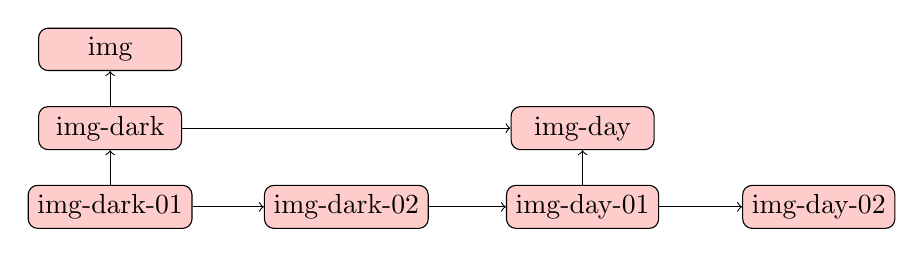
\begin{tikzpicture}
[
    level distance=4cm,
    level 1/.style={sibling distance=5cm},
    level 2/.style={sibling distance=2.5cm},
    level 3/.style={sibling distance=1cm},
    every node/.style={shape=rectangle, rounded corners=.8ex, draw, fill = red!20},
    bigbox/.style={shape=rectangle, rounded corners=.8ex, draw, fill=blue!20, minimum, height=3cm, minimum width=9cm},
]

\node(ik1) at (-4.5,-1){img-dark-01};
\node(ik2) at (-1.5,-1) []{img-dark-02};
\node(id1) at (1.5,-1) []{img-day-01};
\node(id2) at (4.5,-1) []{img-day-02};
\draw[->] (ik1) to (ik2);
\draw[->] (ik2) to (id1);
\draw[->] (id1) to (id2);

\node(ik) at (-4.5,0)[minimum width=12ex]{img-dark};
\node(id) at (1.5,0) [minimum width=12ex]{img-day};
\draw[->] (ik) to (id);

\node(i) at (-4.5,1)[minimum width=12ex]{img};

\draw[->] (ik) to (i);
\draw[->] (ik1) to (ik);
\draw[->] (id1) to (id);

\end{tikzpicture}